\section{El elemento en su posición}

La implementación de todos los algoritmos realizados es de la forma:
\begin{description}
 \item[Entrada:] Vector \texttt{v} y su tamaño \texttt{n}
 \item[Salida:] Entero no negativo que indica el $i$ tal que $v[i]=i$ en caso de que exista o $-1$ en otro caso
\end{description}

En el caso del algoritmo recursivo necesitamos un parámetro adicional para pasar información adicional, pero utilizamos una función \textit{wrapper} que incializa este parámetro adecuadamente.

\subsection{Descripción de los algoritmos y eficiencia teórica}

El algoritmo \textbf{obvio} que resuelve el problema de \textit{El elemento en su posición} consiste
en recorrer cada elemento del vector y comprobar para cada uno de estos si se cumple la
condición deseada ($v[i] = i$):

% Versión obvia
\lstinputlisting[firstline=23, lastline=28]{cpps/posicion.cpp}

Las condiciones de comienzo, actualización y final del bucle son todas $O(1)$, así como el código del interior del bucle. El bucle se ejecutará un máximo de \texttt{n} veces, por lo que es claro que la eficiencia de este algoritmo es de $\mathbf{O(n)}$.

\vspace*{1cm}
\hrulefill
\vspace*{1cm}

Para el algoritmo \textbf{divide y vencerás} hemos realizado dos versiones. La primera de ellas realiza el algoritmo de forma recursiva mientras que la segunda de forma no recursiva. Dada la similitud de nuestro problema con la búsqueda en un vector, nos hemos inspirado en la búsqueda binaria para realizar el siguiente algoritmo:

% Versión recursiva
\lstinputlisting[firstline=60, lastline=77]{cpps/posicion.cpp}

El parámetro \texttt{ajuste} nos sirve para ajustar la comprobación de la posición en función de la posición en la que estemos en el vector.
El caso base utiliza el algoritmo obvio ajustado (la condición que se comprueba es en este caso $v[i]-ajuste == i$), y se utiliza para los vectores de tamaño $\leq 3$, (el umbral encontrado en la siguiente sección).

Si el tamaño del vector es mayor que 3, comprobamos (ajustando) el elemento en el medio.
Distinguimos 3 casos:

\begin{itemize}
  \item El elemento medio está en su posición. En este caso devolvemos este elemento.
  \item $m < v[m]$ (ajustando). En este caso nos basta comprobar el lado izquierdo del vector, ya que $\forall k > 0, v[m + k] \geq v[m] + k > m + k$.
  \item $m > v[m]$ (ajustando). En este caso basta comprobar el lado derecho por un argumento similar, ya que ya que $\forall k > 0, v[m - k] \leq v[m] - k < m - k$.
\end{itemize}

En caso de que no encontremos el elemento en lado adecuado devolvemos $-1$, que nos indica que no existe ningún elemento en su posición.

La \textbf{eficiencia} teórica de este algoritmo puede calcularse a partir de su ecuación de recurrencia, de la forma:

\[
T(n) = \begin{cases} T(n/2) + O(1) & \mbox{si } n > 3 \\
O(1) & \mbox{si } n \leq 3 \end{cases}\]

Sustituyendo $n = 2^k$ obtenemos que el orden de eficiencia de este algoritmo es $\mathbf{O(\log(n))}$.

\vspace*{1cm}
\hrulefill
\vspace*{1cm}

La versión no recursiva:

% Versión no recursiva
\lstinputlisting[firstline=89, lastline=115]{cpps/posicion.cpp}


Es la misma idea que la del algoritmo recursivo, dividiendo el vector en trozos más pequeños, sólo que para hacerlo iterativamente necesitamos un bucle $while$ y unos límites que controlen las dimensiones de los trozos con los que nos vamos quedando del vector, llamados $tope\_min$ y $tope\_max$.  Si encontramos un número que coincida con su posición, devolvemos el número. Si no lo encontramos (muy necesaria la comprobación $tope\_max$ $>=$ $tope\_min$), se devuelve -1.


Al ser la misma idea que el algoritmo recursivo, pero de forma iterativa, la $eficiencia$ teórica es la misma. Es decir, es  $\mathbf{O(\log(n))}$.

\subsection{Determinación del umbral}

En el caso del algoritmo divide y vencerás hemos hecho un estudio del mismo para determinar el umbral para el caso base (para el cual utilizamos el algoritmo obvio) que resulta más eficiente.

%% TODO: (Antonio) Estudio del umbral

Hemos buscado el punto de corte entre ambos algoritmos, para ver cuándo el algoritmo obvio empieza a ser menos eficiente que el divide y vencerás. Para sacar los datos del lineal no hemos tenido problemas, pero sí surgieron errores cuando queríamos compararlo con el divide y vencerás, que tardaba demasiado poco, y cualquier mínimo error movía la gráfica lo suficiente para que no se pudiera determinar nada.

Para poder estabilizar los datos y poder compararlos tuvimos que realizar una media de medio millón de ejecuciones, y realizar la gráfica de esos datos. Los datos de las ejecuciones son los siguientes:

\vspace*{1cm}

\pgfplotstableread{dats/posicion_t_50.dat}\posObvioComp
\pgfplotstableread{dats/posicion_1_50.dat}\posDyVComp
%\pgfplotstableread{dats/comp_umbral_posicion/posicion_2.dat}\posDyVTwo
\pgfplotstablecreatecol[copy column from table={\posDyVComp}{[index] 1}] {par1} {\posObvioComp}
%\pgfplotstablecreatecol[copy column from table={\posDyVTwo}{[index] 1}] {par2} {\posObvio}

\pgfplotstabletypeset[
display columns/0/.style={column name=Tamaño},
display columns/1/.style={column name=Algoritmo Obvio},
display columns/2/.style={column name=Algoritmo DyV (rec)}
%display columns/3/.style={column name=Algoritmo DyV (no rec)},
]{\posObvioComp}

\vspace*{1cm}

Y las gráficas que muestran los datos:
\begin{figure}[H]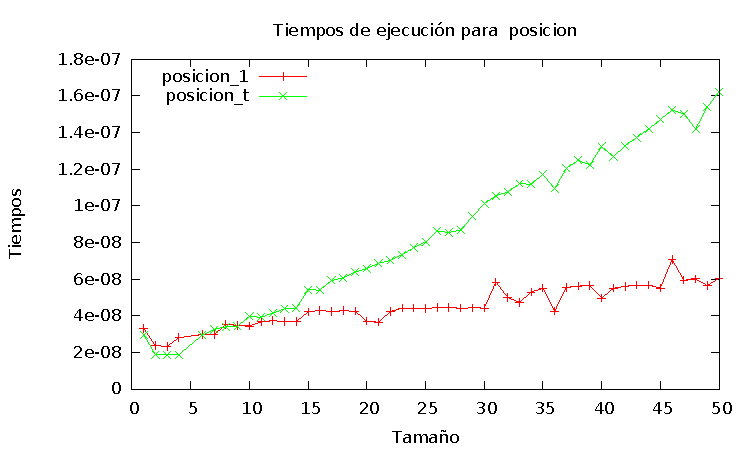
\includegraphics[width=13cm]{img/posicion_todos1_g_50.pdf} \centering
	\caption{Comparativa de tiempos en tamaños chicos para ver el umbral óptimo}\end{figure}

Vimos que el punto de corte estaba cerca del 6, aunque luego cuando estuvimos probando umbrales, el óptimo apareció en el 3, como se verá justo a continuación.

\subsection{Comparación de algoritmos}

A continuación mostramos las tablas y gráficas de comparaciones de diferentes umbrales, junto a sus funciones híbridas. Cogimos los umbrales cercanos al punto de corte anteriormente mencionado:

\vspace*{1cm}

\pgfplotstableread{dats/comp_umbral_posicion/posicion_t.dat}\posObvioCompUmbral
\pgfplotstableread{dats/comp_umbral_posicion/posicion_1.dat}\posDyVUmbralOne
\pgfplotstableread{dats/comp_umbral_posicion/posicion_1_umbral_2.dat}\posDyVUmbralTwo
\pgfplotstableread{dats/comp_umbral_posicion/posicion_1_umbral_3.dat}\posDyVUmbralThree
\pgfplotstableread{dats/comp_umbral_posicion/posicion_1_umbral_4.dat}\posDyVUmbralFour
\pgfplotstableread{dats/comp_umbral_posicion/posicion_1_umbral_5.dat}\posDyVUmbralFive
\pgfplotstablecreatecol[copy column from table={\posDyVUmbralOne}{[index] 1}] {par1} {\posObvioCompUmbral}
\pgfplotstablecreatecol[copy column from table={\posDyVUmbralTwo}{[index] 1}] {par2} {\posObvioCompUmbral}
\pgfplotstablecreatecol[copy column from table={\posDyVUmbralThree}{[index] 1}] {par3} {\posObvioCompUmbral}
\pgfplotstablecreatecol[copy column from table={\posDyVUmbralFour}{[index] 1}] {par4} {\posObvioCompUmbral}
\pgfplotstablecreatecol[copy column from table={\posDyVUmbralFive}{[index] 1}] {par5} {\posObvioCompUmbral}

\pgfplotstabletypeset[
display columns/0/.style={column name=Tamaño},
display columns/1/.style={column name=Algoritmo Obvio},
display columns/2/.style={column name=Umbral 1},
display columns/3/.style={column name=Umbral 2},
display columns/4/.style={column name=Umbral 3},
display columns/5/.style={column name=Umbral 4},
display columns/6/.style={column name=Umbral 5},
skip rows between index={25}{50}
]{\posObvioCompUmbral}

\vspace*{1cm}

Y las gráficas de los mismos:

\begin{figure}[H]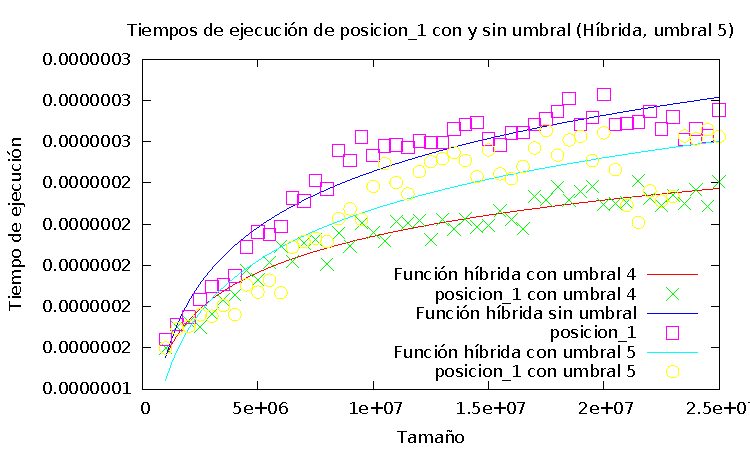
\includegraphics[width=13cm]{img/posicion_1_comparativa_umbral2.pdf} \centering
	\caption{Tiempos y funciones híbridas de umbrales 4 y 5}\end{figure}

Como poner los 5 umbrales y sus híbridas haría que la gráfica fuera un poco caótica, hemos decidido poner una gráfica solo con las híbridas de los algoritmos, para que se vea la tendencia de los tiempos, que es lo que importa:

\begin{figure}[H]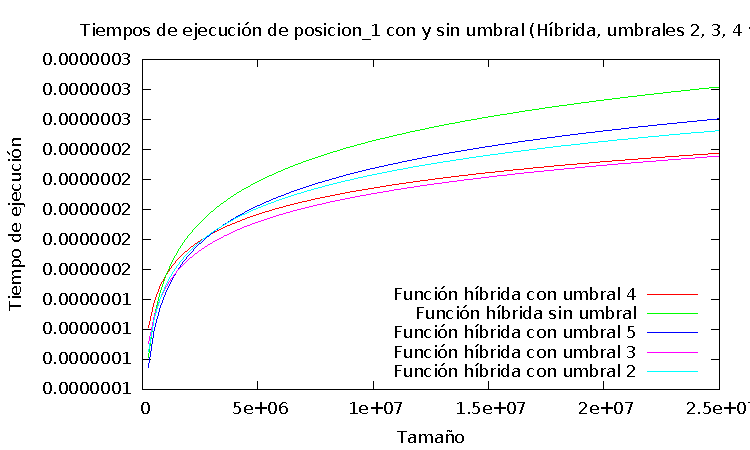
\includegraphics[width=13cm]{img/posicion_1_comparativa_umbral5.pdf} \centering
	\caption{Tiempos y funciones híbridas de umbrales 2, 3, 4 y 5}\end{figure}

En la gráfica ya podemos observar que el umbral 3 y 2 son prácticamente iguales, y los preferibles. La gráfica va aumentando conforme nos alejamos de estos dos números, como se puede ver que los umbrales 4 y 5 se encuentran un poco más arriba.

Hemos conseguido bajar un cuarto el tiempo de ejecución solo jugando con el umbral, así que remarcamos la importancia de encontrar el óptimo en un algoritmo Divide y Vencerás.

Por último colocamos una gráfica 3D de cómo varían los tiempos en función del umbral y del tamaño.

\begin{figure}[H]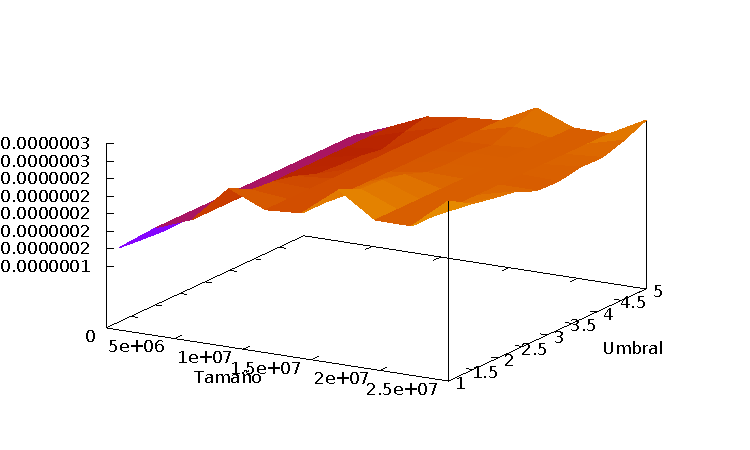
\includegraphics[width=13cm]{img/umbral_posicion.pdf} \centering
	\caption{Tiempos según Umbral y Tamaño}\end{figure}

\subsection{Eficiencia empírica de los algoritmos}

Utilizando la librería \texttt{chrono} hemos medido los tiempos de los algoritmos para un conjunto fijo de tamaños. Aunque los algoritmos son rápidos para tamaños grandes, las funciones auxiliares utilizadas para la generación de muestras aleatorias que permitan medir el tiempo han dificultado la obtención de los datos. Los datos obtenidos pueden verse en la siguiente tabla:


% tex.stackexchange.com/questions/10284

\vspace*{1cm}

\pgfplotstableread{dats/comp_umbral_posicion/posicion_t.dat}\posObvio
\pgfplotstableread{dats/comp_umbral_posicion/posicion_1.dat}\posDyV
%\pgfplotstableread{dats/comp_umbral_posicion/posicion_2.dat}\posDyVTwo
\pgfplotstablecreatecol[copy column from table={\posDyV}{[index] 1}] {par1} {\posObvio}
%\pgfplotstablecreatecol[copy column from table={\posDyVTwo}{[index] 1}] {par2} {\posObvio}

\pgfplotstabletypeset[
display columns/0/.style={column name=Tamaño},
display columns/1/.style={column name=Algoritmo Obvio},
display columns/2/.style={column name=Algoritmo DyV (rec)},
skip rows between index={25}{50}
%display columns/3/.style={column name=Algoritmo DyV (no rec)},
]{\posObvio}

\vspace*{1cm}

Podemos ajustar estos datos con una función representativa del orden de eficiencia teórico obtenido en la sección anterior:

%% TODO: (¿?) Ajustes de las funciones

En el siguiente gráfico podemos observar además una comparativa de las eficiencias empíricas y teóricas de los algoritmos realizados:



%% TODO: (Antonio) Gráfica con todos los algoritmos

\subsection{Vectores con elementos repetidos}

En el caso de que tengamos elementos repetidos el razonamiento realizado para justificar el algoritmo divide y vencerás no es válido, y es sencillo encontrar ejemplos de vectores con elementos en su posición para los cuales nuestro algoritmo no funciona.

Consideremos por ejemplo el caso del vector $v = [1,2,2]$. $1 <v[1]$, por lo que nuestro algoritmo comprobaría sólo el lado izquierdo ($[1]$) y no encontraría el elemento en la posición 2, que está en su posición.

Podemos plantear otro algoritmo de carácter similar para encontrar un elemento en su posición en estos casos:

\lstinputlisting[firstline=126, lastline=150]{cpps/posicion.cpp}

Este algoritmo realiza la búsqueda en el mismo orden en el que la haría el recursivo, solo que si no encuentra el número, hace también la otra mitad del vector. Este comportamiento provoca que se comporte casi logarítmico cuando hay un elemento en su posición, y peor que lineal cuando no se encuentra.

Por tanto, la eficiencia de este algoritmo depende drásticamente en la probabilidad de que un elemento esté en su posición y en la probabilidad de repetidos. Cuando más repetidos y menos en su posición, peor. Como en una distribución uniforme sobre el rango de elementos en los que trabajamos la probabilidad de que un elemento caiga en su posición es bastante baja, por mucho que a veces sea logarítmico, no compensa las veces que es peor que lineal.

Para comparar este algoritmo con los demás hemos necesitado de nuevo realizar una media de varios miles de ejecuciones para que se pudiera ver de forma decente lo que pasaba. A continuación dejamos las tablas y gráficos que lo muestran:
